\subsection{Massa dell'elettrone}

Per ricavare la massa dell'elettrone misuriamo l'energia del picco di annichilazione del \na{}
calibrando la scala di energia con i fotopicchi di \co{} e \cs{}.
Poiché la scala di energia varia significativamente nell'arco di tempo in cui facciamo le misure,
misuriamo contemporaneamente lo spettro di tutte le sorgenti.
Triggeriamo su un singolo PMT,
collegando solo quel PMT all'ADC, per evitare il crosstalk tra i canali dell'ADC.
Ripetiamo la misura con i 3 scintillatori disponibili.

\subsubsection{Fit dei picchi}

\begin{figure}
	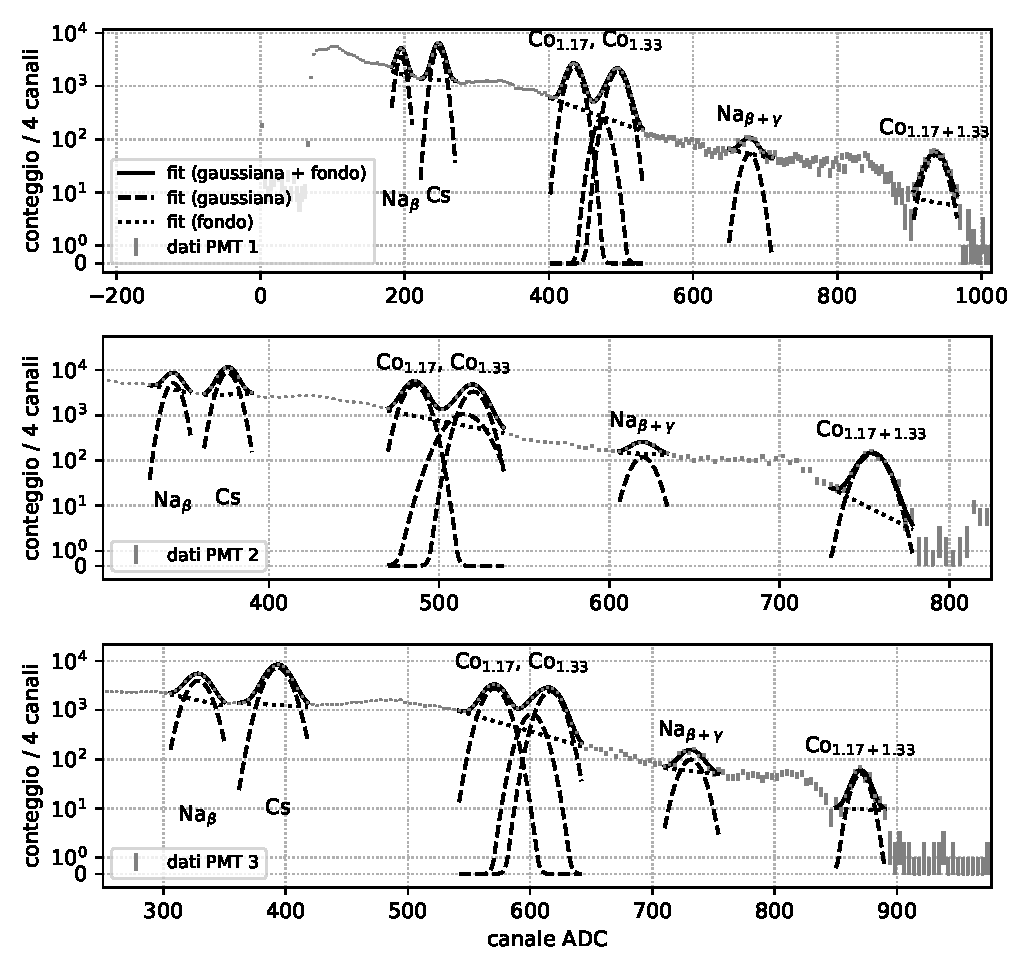
\includegraphics[width=\textwidth]{immagini/mass18-peaks}
	\caption{\label{fig:mass18-peaks}
	Ciao}
\end{figure}

Fittiamo ogni picco, scegliendo a mano l'intervallo di canali su cui fittare,
con una gaussiana più un esponenziale come fondo.
Il fit è ai minimi quadrati sull'istogramma.
I bin fittati contengono tutti almeno 5 eventi.
Controlliamo che cambiare il ribinnaggio dei canali dell'ADC non cambia significativamente il risultato.
I~fit sono riportati in \autoref{fig:mass18-peaks}.
Tutti i fit hanno un pvalue ragionevole;
il test di Kolmogorov-Smirnov sull'uniformità dei pvalue dà un pvalue \SI{18}\%.
Per i picchi del cobalto e quello del neon, che sono sovrapposti, il fit è unico.
Con dei test vediamo che il risultato per la media del picco del neon,
che è praticamente nascosto da quelli del cobalto,
è instabile, quindi lo teniamo nel fit come fondo ma non lo usiamo per ricavare la massa.

\subsubsection{Fit della massa}

\begin{figure}
	\centering
	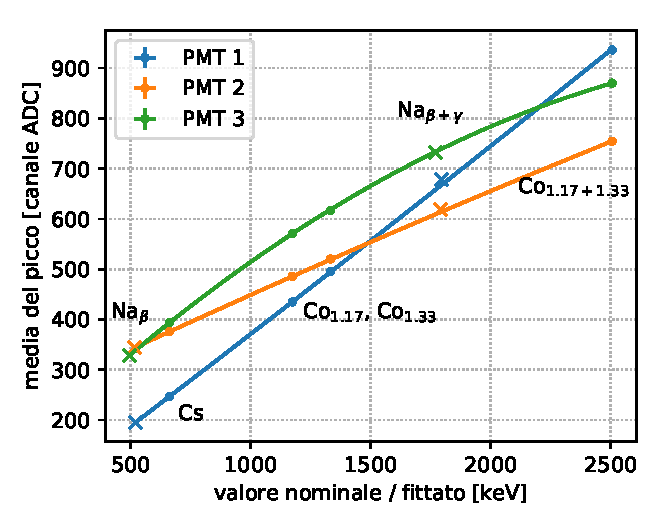
\includegraphics[width=25em]{immagini/mass18-cal}
	\caption{\label{fig:mass18-cal}
	Ciao}
\end{figure}

\begin{table}
	\hspace{-3em}
	\begin{tabular}{c|cccc|cc}
		PMT & $a$ & $b$ [\si{keV^{-1}}] & $c$ [\si{keV^{-2}}] & $m$ [\si{keV}] & $\chi^2$/dof & $F$ \\
		\hline
		1 &   \num{7.31(54)} &  \num{0.3584(11)} &   \num{2.60(26)} & \num{519.95(50)} & 33.3 & 6.9 \\
		2 & \num{228.02(31)} & \num{0.22802(56)} &  \num{-3.55(11)} & \num{516.44(55)} & 24.4 & 6.2 \\
		3 & \num{113.47(44)} & \num{0.46701(84)} & \num{-32.94(18)} & \num{495.25(44)} &  4.1 & 2.3
	\end{tabular}
	\caption{\label{tab:massfit}
	Risultati dei fit di calibrazione e massa dell'elettrone per ogni PMT.
	La curva di calibrazione è $E_\text{adc}=2cE^2+bE+a$.
	In tutti i fit le correlazioni risultano circa \SI{50}\% tra $m$ e gli altri parametri
	e circa \SI{95}\% tra $a$, $b$ e $c$.
	$F$ è il fattore per cui riscalare l'incertezza su $m$
	ricavato testando il fit sui picchi di calibrazione.}
\end{table}

Inizialmente fittiamo le medie dei picchi in funzione dell'energia con una retta
\begin{equation}
	\label{eq:retta}
	E_\text{adc} = b \cdot E + a,
\end{equation}
dove, a seconda dei casi, $E$ è
\begin{itemize}
	\item il valore noto dell'energia per i picchi di calibrazione;
	\item la massa $m$ dell'elettrone (parametro di fit) per il picco di annichilazione;
	\item $m$ più l'energia del fotone del neon per il picco $\na_{\beta+\gamma}$.
\end{itemize}
Nel fit teniamo conto della correlazione tra i picchi del cobalto.
Il pvalue del fit è praticamente 0,
ovvero le incertezze statistiche sono sufficientemente piccole da rigettare il modello \eqref{eq:retta}.

Poiché abbiamo ancora 3 gradi di libertà,
rendiamo il modello più generico aggiungendo il termine quadratico:
\begin{equation}
	\label{eq:parabola}
	E_\text{adc} = 2c \cdot E^2 + b \cdot E + a.
\end{equation}
Anche questo modello viene rigettato con forza per i PMT 1 e 2, ma non per il 3.
Non vogliamo avere meno di due gradi di libertà nel fit,
quindi in mancanza di un modello adeguato stimiamo un'incertezza sistematica aggiuntiva in questo modo:
per ogni picco di calibrazione ripetiamo il fit lasciando libera,
oltre all'energia del picco di annichilazione,
anche l'energia del picco di calibrazione.
Per ognuno di questi fit calcoliamo il rapporto tra
la differenza tra l'energia fittata e l'energia nota del picco di calibrazione
e la deviazione standard stimata dal fit sull'energia fittata.
Riscaliamo l'incertezza sulla massa del fit principale
per la media quadratica di questi rapporti.
Il grafico del fit è riportato in \autoref{fig:mass18-cal},
i risultati dettagliati sono riportati in \autoref{tab:massfit}.
Le masse fittate, con l'incertezza riscalata, risultano
\begin{center}
	\begin{tabular}{cc}
		PMT 1: & $m=\SI{520.0(34)}{keV}$ \\
		PMT 2: & $m=\SI{516.4(34)}{keV}$ \\
		PMT 3: & $m=\SI{495.2(10)}{keV}$
	\end{tabular}
\end{center}
